\documentclass[a4paper,twoside]{article}
\usepackage{blindtext}  
\usepackage{geometry}

% Chinese support
\usepackage[UTF8, scheme = plain]{ctex}

% Page margin layout
\geometry{left=2.3cm,right=2cm,top=2.5cm,bottom=2.0cm}


\usepackage{listings}
\usepackage{xcolor}
\usepackage{geometry}
\usepackage{amsmath}
\usepackage{float}
\usepackage{hyperref}

\usepackage{graphics}
\usepackage{graphicx}
\usepackage{epsfig}
\usepackage{float}
\usepackage{caption}
\usepackage{subcaption}

\usepackage{algorithm}
\usepackage[noend]{algpseudocode}

\usepackage{booktabs}
\usepackage{threeparttable}
\usepackage{longtable}
\usepackage{tikz}
\usepackage{multicol}

% cite package, to clean up citations in the main text. Do not remove.
\usepackage{cite}

\usepackage{color,xcolor}

%% The amssymb package provides various useful mathematical symbols
\usepackage{amssymb}
%% The amsthm package provides extended theorem environments
\usepackage{amsthm}
\usepackage{amsfonts}
\usepackage{enumerate}
\usepackage{enumitem}
\usepackage{listings}
\usepackage{minted}


\usepackage{indentfirst}
\setlength{\parindent}{2em} % Make two letter space in the first paragraph
\usepackage{setspace}
\linespread{1.5} % Line spacing setting
\usepackage{siunitx}
\setlength{\parskip}{0.5em} % Paragraph spacing setting

% \usepackage[contents =22920202204622, scale = 10, color = black, angle = 50, opacity = .10]{background}

\renewcommand{\figurename}{图}
\renewcommand{\listingscaption}{代码}
\renewcommand{\tablename}{表格}
\renewcommand{\contentsname}{目录}
\floatname{algorithm}{算法}

\graphicspath{ {images/} }

%%%%%%%%%%%%%
\newcommand{\StudentNumber}{22920202204622}  % Fill your student number here
\newcommand{\StudentName}{熊恪峥}  % Replace your name here
\newcommand{\PaperTitle}{实验(五)磁盘、固态盘仿真}  % Change your paper title here
\newcommand{\PaperType}{计算机系统结构实验} % Replace the type of your report here
\newcommand{\Date}{2023年5月20日}
\newcommand{\College}{信息学院}
\newcommand{\CourseName}{计算机系统结构}
%%%%%%%%%%%%%

%% Page header and footer setting
\usepackage{fancyhdr}
\usepackage{lastpage}
\pagestyle{fancy}
\fancyhf{}
% This requires the document to be twoside
\fancyhead[LO]{\texttt{\StudentName }}
\fancyhead[LE]{\texttt{\StudentNumber}}
\fancyhead[C]{\texttt{\PaperTitle }}
\fancyhead[R]{\texttt{第{\thepage}页,共\pageref*{LastPage}页}}


\title{\PaperTitle}
\author{\StudentName}
\date{\Date}

\algnewcommand\algorithmicinput{\textbf{Input:}}
\algnewcommand\algorithmicoutput{\textbf{Output:}}
\algnewcommand\Input{\item[\algorithmicinput]}%
\algnewcommand\Output{\item[\algorithmicoutput]}%

\usetikzlibrary{positioning, shapes.geometric}

\begin{document}
	
%%%%%%%%%%%%%%%%%%%%%%%%%%%%%%%%%%%%%%%%%%%%
\makeatletter % change default title style
\renewcommand*\maketitle{%
	\begin{center} 
		\bfseries  % title 
		{\LARGE \@title \par}  % LARGE typesetting
		\vskip 1em  %  margin 1em
		{\global\let\author\@empty}  % no author information
		{\global\let\date\@empty}  % no date
		\thispagestyle{empty}   %  empty page style
	\end{center}%
	\setcounter{footnote}{0}%
}
\makeatother
%%%%%%%%%%%%%%%%%%%%%%%%%%%%%%%%%%%%%%%%%%%%
	
	
\thispagestyle{empty}

\vspace*{1cm}

\begin{figure}[htb]
	\centering
	
\includegraphics[width=4.0cm]{logo.png}
\end{figure}

\vspace*{1cm}

\begin{center}
	\Huge{\textbf{\PaperType}}
	
	\Large{\PaperTitle}
\end{center}

\vspace*{1cm}

\begin{table}[H]
	\centering	
	\begin{Large}
		\renewcommand{\arraystretch}{1.5}
		\begin{tabular}{p{3cm} p{5cm}<{\centering}}
			姓\qquad 名 & \StudentName  \\
			\hline
			学\qquad号 & \StudentNumber \\
			\hline
			日\qquad期 & \Date  \\
			\hline
			学\qquad院 & \College  \\
			\hline
			课程名称 & \CourseName  \\
			\hline
		\end{tabular}
	\end{Large}
\end{table}

\newpage

\title{
	\Large{\textcolor{black}{\PaperTitle}}
}
	
	
\maketitle
	
\tableofcontents
 
\newpage
\setcounter{page}{1}

\begin{spacing}{1.2}

\section{测试RAID0、RAID1、RAID5的性能}

为了比较RAID0、RAID1、RAID5的性能,首先需要保证具有相同的有效盘数。
假设具有4个有效磁盘。RAID0采用条带化,因此没有冗余磁盘,需要4个磁盘。
RAID1采用对每个磁盘进行镜像,因此需要8个磁盘。
RAID5需要存储校验信息,因此需要5个磁盘。如图~\ref{fig:raids}。
\begin{figure}[h]
	\centering
	\caption{磁盘布局}
	\label{fig:raids}
	\begin{subfigure}{0.35\textwidth}
		\centering
		\caption{RAID0}
		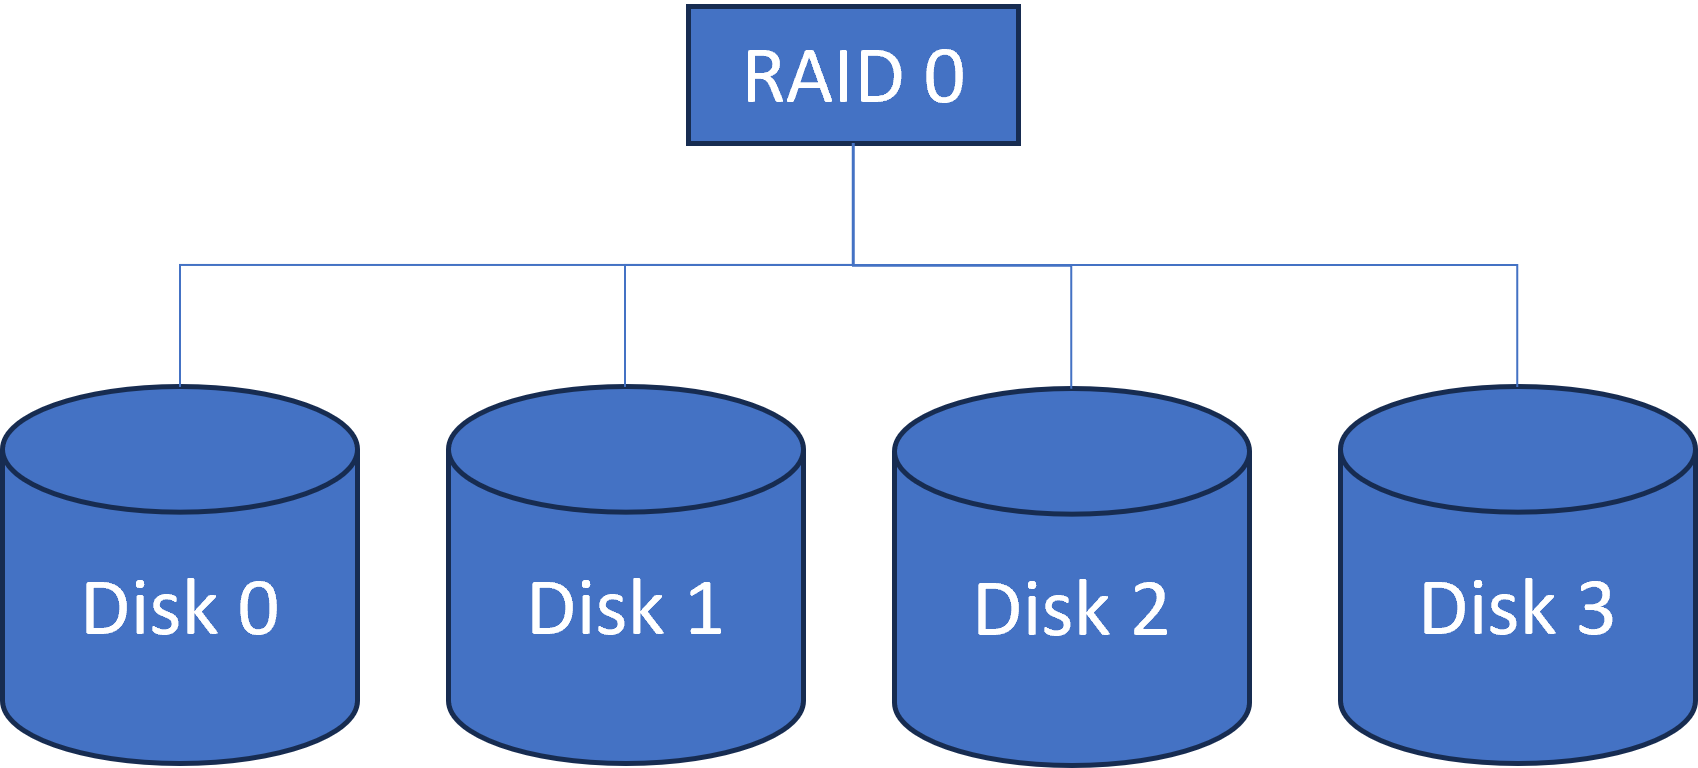
\includegraphics[width=0.9\linewidth]{raid0.png}
	\end{subfigure}
	\begin{subfigure}{0.45\textwidth}
		\centering
		\caption{RAID5}
		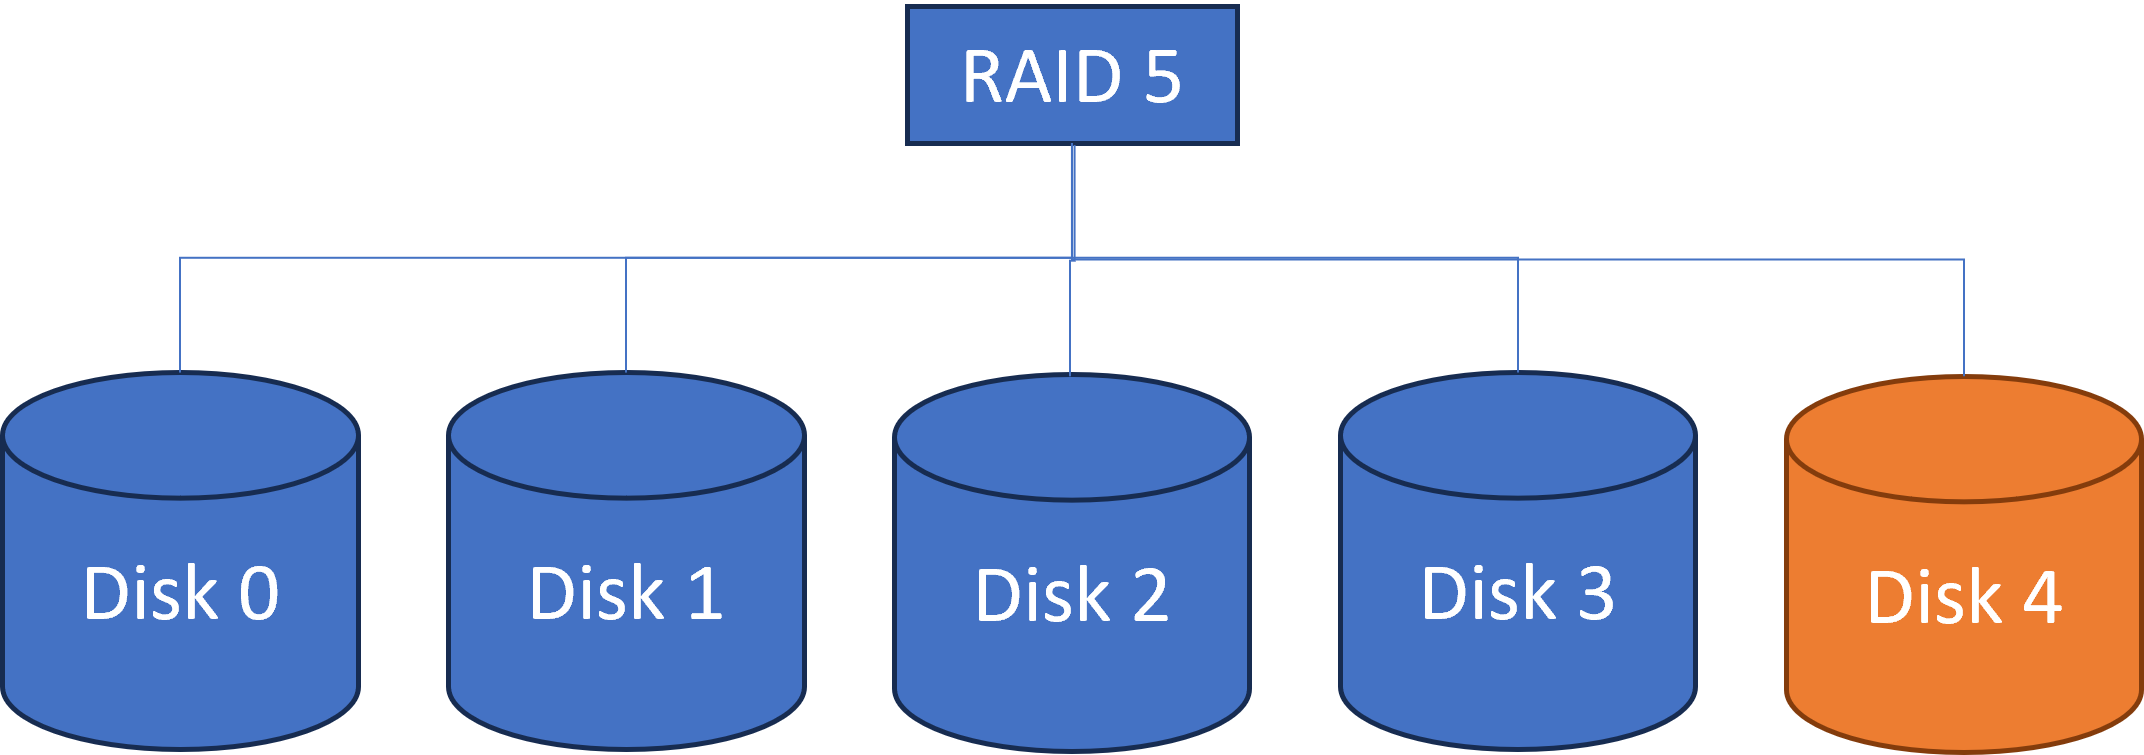
\includegraphics[width=0.9\linewidth]{raid5.png}
	\end{subfigure}
	\begin{subfigure}{0.6\textwidth}
		\centering
		\caption{RAID1}
		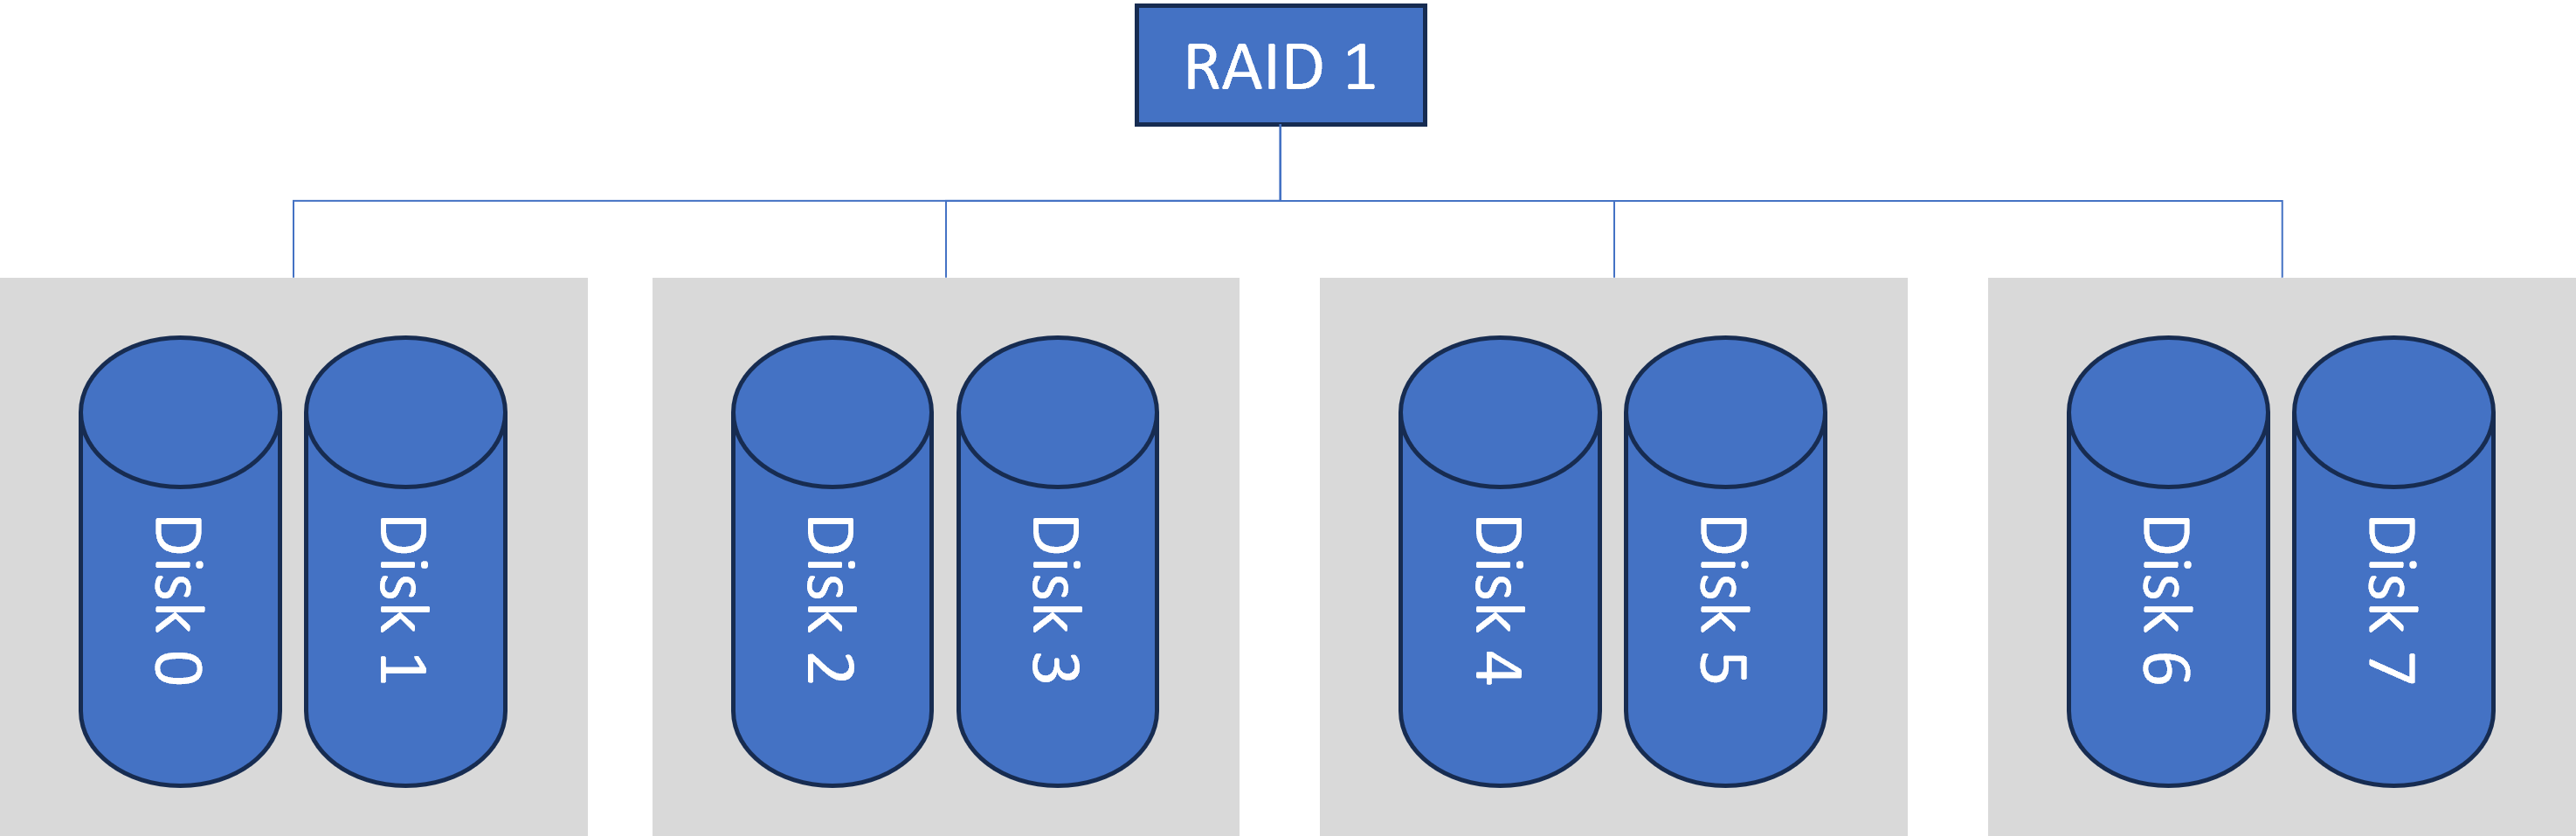
\includegraphics[width=0.9\linewidth]{raid1.png}
	\end{subfigure}
\end{figure}

根据上图调整配置文件中的\texttt{disksim\_logorg}结构。就可以进行公平的比较。

\subsection{实验结果}
实验结果如图。分别使用Synthetic负载和真实负载Financial1\_10k。
Synthetic负载的输出如图~\ref{fig:synout}。
\begin{figure}[h]
	\centering
	\caption{Synthetic负载的输出}
	\label{fig:synout}
	\begin{subfigure}{0.45\textwidth}
		\centering
		\caption{RAID0}
		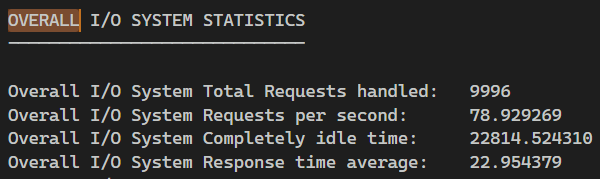
\includegraphics[width=0.9\linewidth]{out0.png}
	\end{subfigure}
	\begin{subfigure}{0.45\textwidth}
		\centering
		\caption{RAID1}
		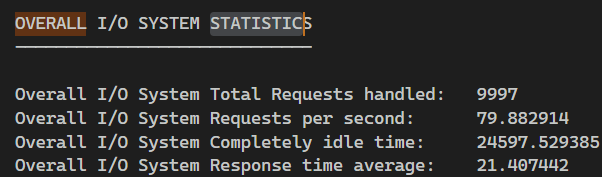
\includegraphics[width=0.9\linewidth]{out1.png}
	\end{subfigure}
	\begin{subfigure}{0.45\textwidth}
		\centering
		\caption{RAID5}
		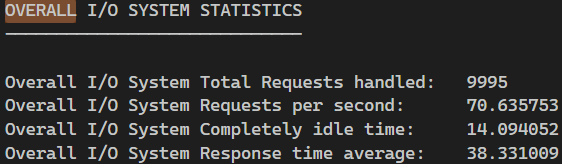
\includegraphics[width=0.9\linewidth]{out5.png}
	\end{subfigure}
\end{figure}
所有结果如表~\ref{tbl:res},可视化如图~\ref{fig:vis}
\begin{table}[h]
	\centering
	\caption{实验结果}
	\label{tbl:res}
	\begin{tabular}{c|c|c|c}
		\toprule
		\hline
		& RAID0 & RAID1 & RAID5 \\ \hline
		Synthetic & 22.954379 & 21.407442 & 38.331009 \\
		\hline
		Financial1\_10k & 1547.141826 & 1433.574369	& 7930.652398		\\ 
		\hline
		\bottomrule
	\end{tabular}
\end{table}
\begin{figure}[ht]
	\centering
	\caption{结果可视化}
	\label{fig:vis}
	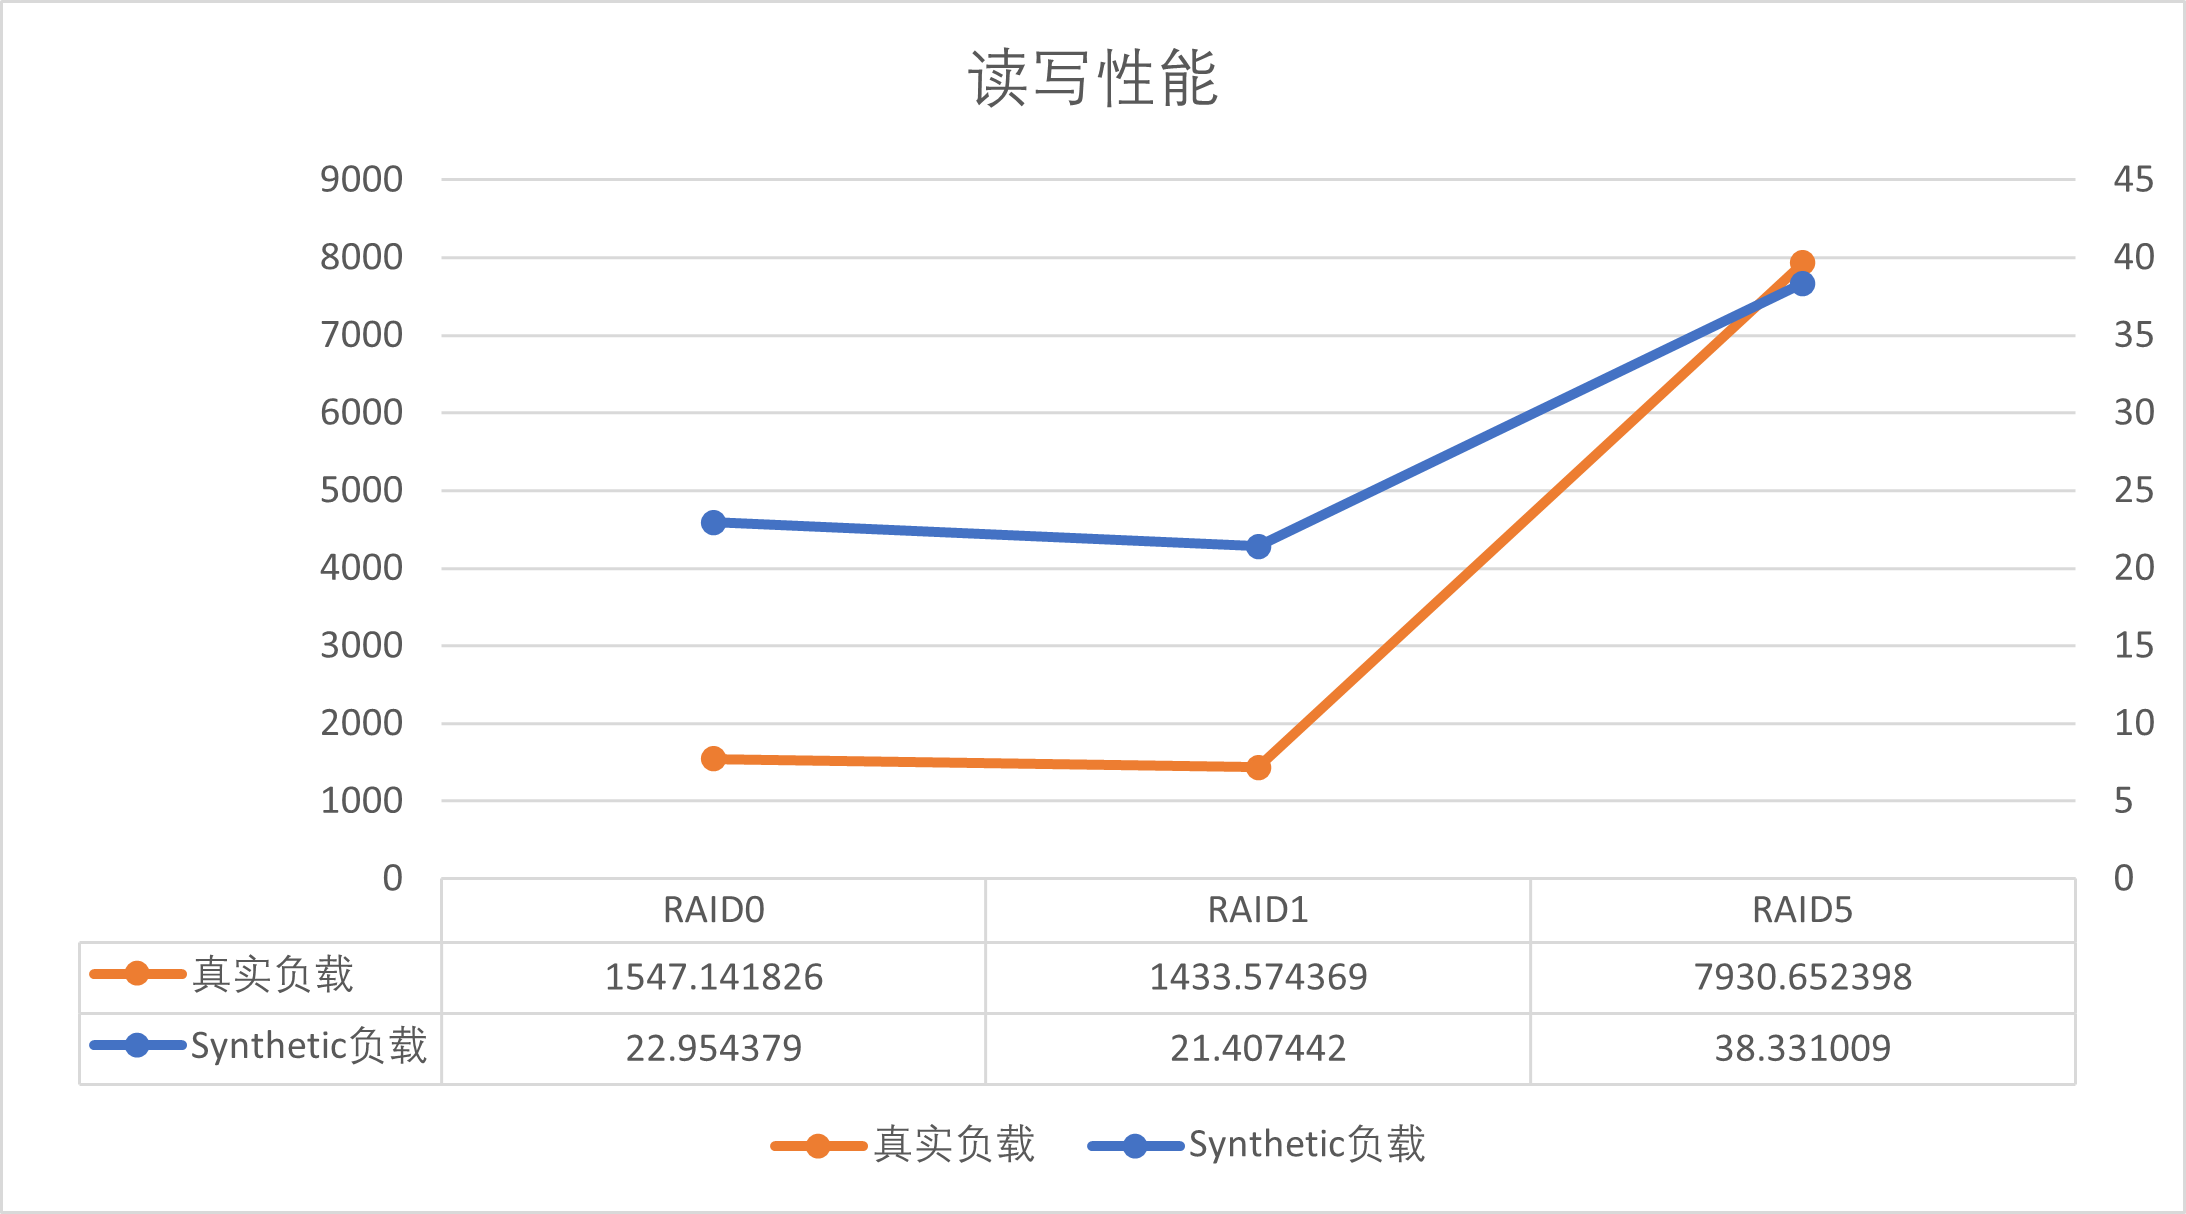
\includegraphics[width=0.6\linewidth]{res.png}
\end{figure}
从中可以得出结论,RAID5最慢,RAID0和RAID1较快,但RAID1具有更快的速度。

\section{探究实验:分析验证参数敏感性}

我选用RAID5测试参数的敏感性,参数包括盘数,条带大小。
为了测试盘数,可以通过修改参数\texttt{devices}来修改盘数。
为了测试条带大小,需要修改\texttt{Stripe unit}和\texttt{Parity stripe unit}。
根据disksim的文档,以上两项参数最好设置成同一数值,因为不同的数值在当前版本中没有经过测试:
\begin{quotation}
The parity stripe unit size does not have to be equal
to the stripe unit size, but one must be a multiple of the other. Use of non-equal stripe unit
sizes for data and parity has not been thoroughly tested in the current release of DiskSim.
\end{quotation}

为了方便测试,我使用Shell脚本自动化地运行多个测试,如代码~\ref{code:ss}。
\begin{listing}[htb]
	\caption{Shell脚本自动化地运行多个测试}
	\label{code:ss}
	\begin{minted}{shell}
for input in 'raid5n5' 'raid5n6' 'raid5n7' 'raid5n8' 'raid5n9'
do
echo $input.parv
../src/disksim $input.parv $input.syn.outv ascii 0 1
../src/disksim $input.parv $input.real.outv ascii Financial1_10k.ascii 0
done

for input in 'raid5s64' 'raid5s128' 'raid5s256' 'raid5s512' 'raid5s1024'
do
echo $input.parv
../src/disksim $input.parv $input.syn.outv ascii 0 1
../src/disksim $input.parv $input.real.outv ascii Financial1_10k.ascii 0
done
	\end{minted}
\end{listing}

运行测试的结果如图~\ref{fig:res2}。
可以发现,如图~\ref{fig:dcnt},访问时间和盘数具有负相关的关系。随着盘数的升高,访问时间逐步下降。
因此,RAID5对盘数这一参数具有比较高的敏感性。

如图~\ref{fig:ssize},随着条带大小的增加,访问时间逐步下降。但是,当条带大小达到一定程度后,访问时间不再下降,反而上升。
因此RAID5对条带大小这一参数也具有一定的敏感性。但是敏感性不如盘数。因为没有形成特定的相关关系。
\begin{figure}[ht]
	\centering
	\caption{参数敏感性的结果}
	\label{fig:synout}
	\begin{subfigure}{0.45\textwidth}
		\centering
		\caption{盘数}
		\label{fig:dcnt}
		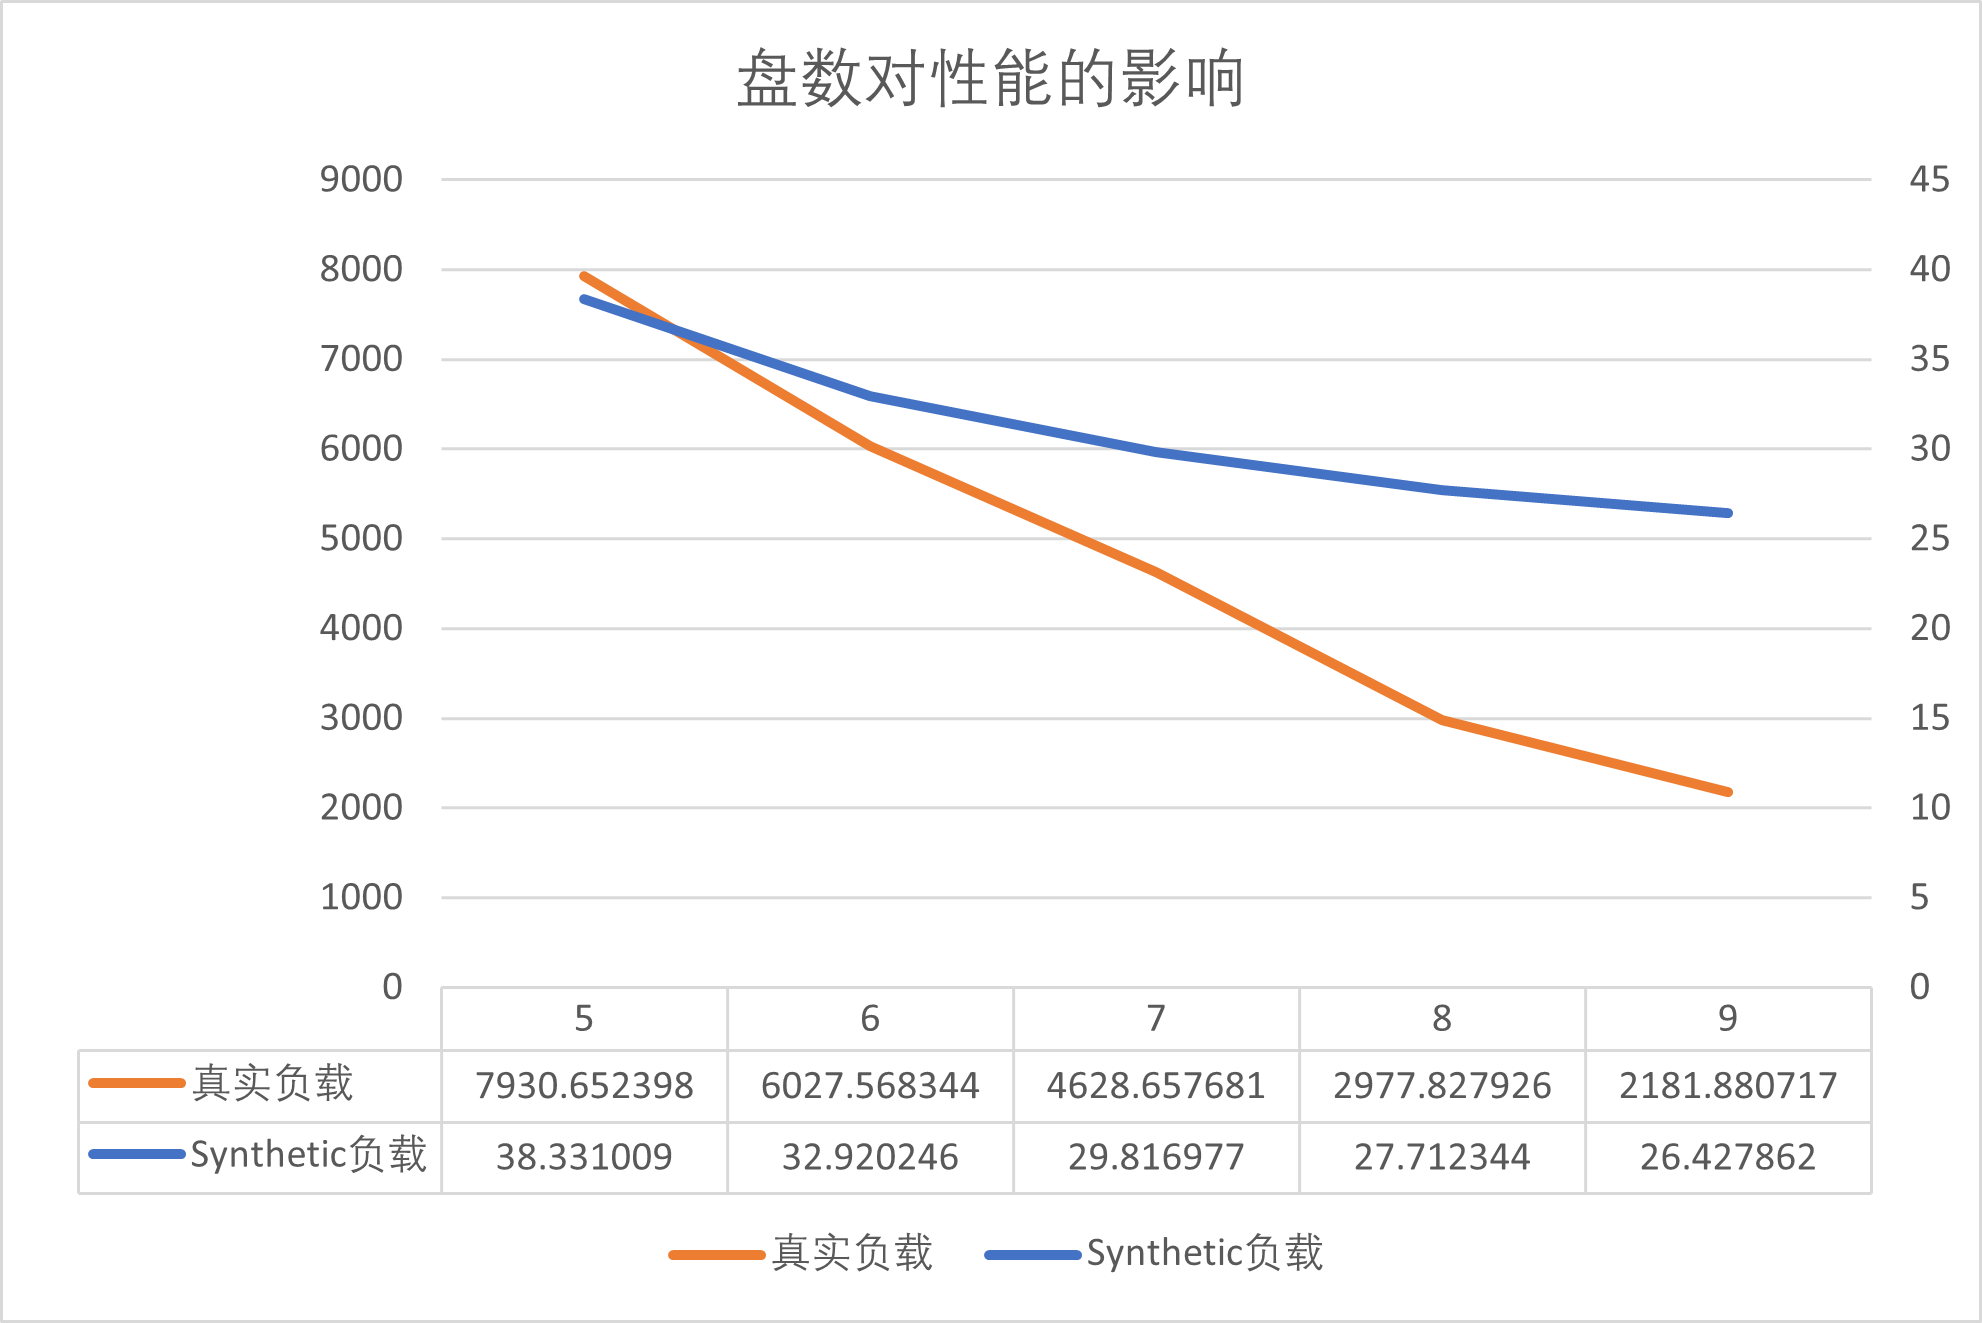
\includegraphics[width=0.9\linewidth]{dcnt.png}
	\end{subfigure}
	\begin{subfigure}{0.45\textwidth}
		\centering
		\caption{条带大小}
		\label{fig:ssize}
		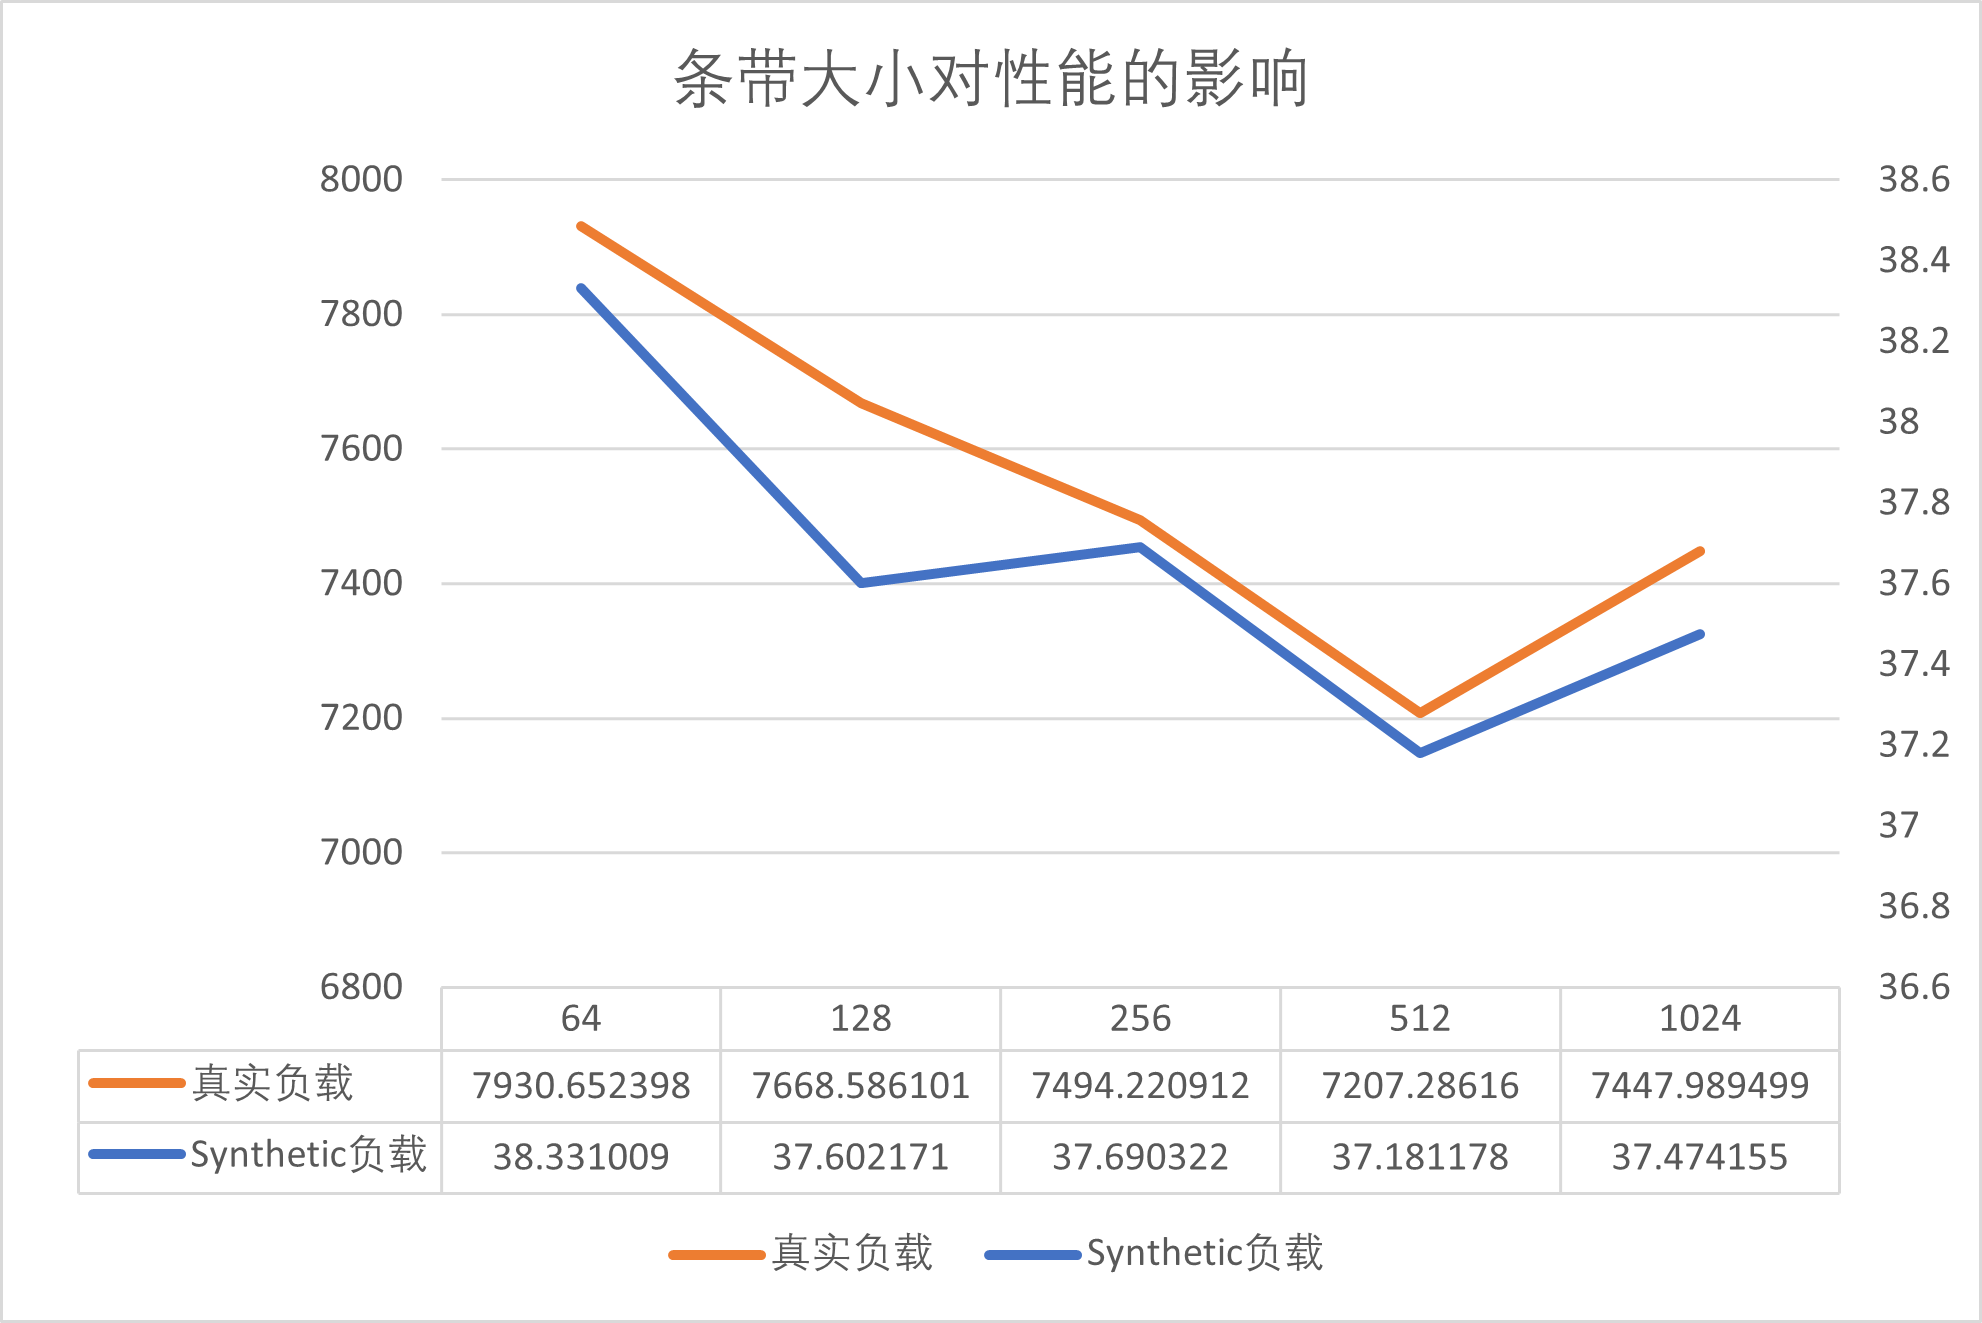
\includegraphics[width=0.9\linewidth]{ssize.png}
	\end{subfigure}
\end{figure}

\section{思考题}
考虑以下应用场景,选择你认为合适的RAID设计。
\begin{enumerate}
\item 非线性编辑工作站(做视频编辑的电脑):
应该使用RAID0,编辑视频需要大量的存储访问,并且要求访问速度快。在使用时应该使用较大的条带大小,以提高访问速度。
\item web服务器:
应该使用RAID1,这样可以保证损坏时仍然可以工作。
\item 代理服务器:
应该使用RAID1,这样可以保证损坏时仍然可以工作。
\item FTP服务器:
应该使用RAID1,这样能更好保障文件安全,并且和RAID5相比也有较高的读写速度。
\item 一卡通帐户数据服务器:
应该使用RAID5,一卡通账户对数据的正确性要求高,RAID5可以更好地保障完整性。
\end{enumerate}


\end{spacing}

\end{document}